\chapter{Testy aplikacji}
W celu zapewnienia poprawności działania aplikacji stworzono zestaw testów jednostkowych
sprawdzających poprawność działania najważniejszych komponentów systemu. 
Wykorzystano bibliotekę XUnit służącą do tworzenia testów jednostkowych w technologii .NET
oraz bibliotekę Moq służącą do przygotowania danych testowych oraz zastąpieniu nim konkretnych implementacji.
Pokryty został kod odnoszący się do logiki biznesowej, tj. tworzenie modeli, ich modyfikacja
oraz system weryfikacji odczytów. W tej warstwie aplikacji 99\% linii kodu zostało pokryte
testami jednostkowymi, jedynym odstępem jest funkcja obliczająca hash obiektu.
Wygenerowany raport został przedstawiony na Rys. \ref{core:coverage}.
\begin{figure}[h!]
  \centering
  \includegraphics[width=\textwidth]{core_coverage}
  \caption{Procent linii pokrytych testami jednostkowymi w projekcie zawierającym logikę aplikacji}
  \label{core:coverage}
\end{figure}
Dodatkowo pokryte testami zostały serwisy z bardziej zaawansowaną logiką. Większość z nich to proste
warstwy abstrakcji bezpośrednio odwołujące się do innych bibliotek, ale niektóre z nich mają bardziej
skomplikowaną logikę. Takimi klasami są \textbf{JwtTokenProvider} zajmujący się tworzeniem oraz walidacją
tokenów JWT oraz \textbf{ConfigService} zawierający logikę konwertującą wartość tekstową zasad sprawdzania
odczytów na ekspresje środowiska .NET. Obydwa serwisy zostały pokryte w więcej niż 90\% testami jednostkowymi
co zostało przedstawione w reporcie na Rys. \ref{services:coverage}.
\begin{figure}[h!]
  \centering
  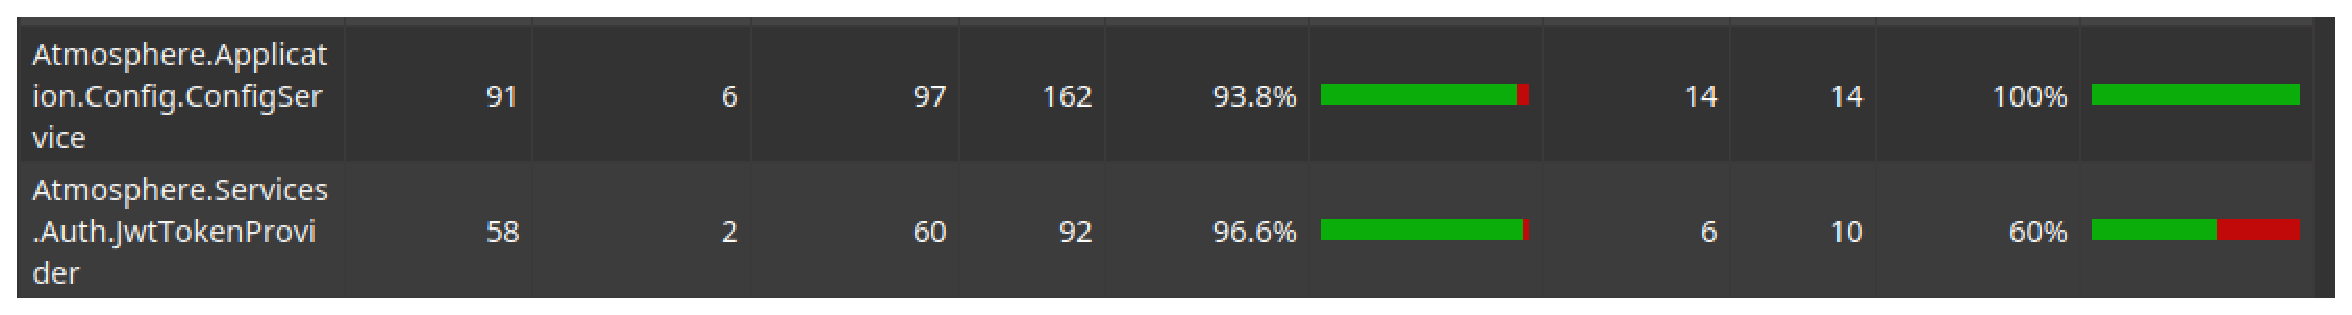
\includegraphics[width=\textwidth]{services_coverage}
  \caption{Procent linii pokrytych testami jednostkowymi w klasach \textbf{JwtTokenProvider} i \textbf{ConfigService}}
  \label{services:coverage}
\end{figure}
Warstwa zawierająca kontrolery nie wymagała testów - zawiera jedynie definicje punktów dostępu.
które wysyłają dalej zapytanie do warstwy aplikacyjnej poprzez wykorzystanie biblioteki MediatoR
oraz kod rejestrujący serwisy.

Wykonano również ręczne testy funkcjonalne aplikacji. Skupiły się głównie na testowaniu aplikacji klienckiej
i jej funkcjonalności. Wykonano wdrożenie systemu używając czystej bazy danych. Pierwszym krokiem
testów było zalogowanie się na konto administratora wykorzystując domyślne login oraz hasło
zdefiniowane w plikach konfiguracyjnych serwera. Następnym krokiem były testy konfiguracji systemu.
Pierwszym parametrem, który uległ zmianie było dodanie nowej reguły walidacji. Wykorzystano
prostą regułę sprawdzającą czy temperatura powietrza wynosi powyżej 22 stopnie Celsjusza, co było
przydatne w następnych testach powiadomień. Do konfiguracji wiadomości email użyto darmowej
bramki smtp.freesmtpservers.com pozwalającą na darmowe testowanie systemów email. 
Wynik tego kroku został przedstawiony na Rys. \ref{test:config}.
\begin{figure}[h!]
  \centering
  \includegraphics[width=\textwidth]{test_config}
  \caption{Testowa konfiguracja}
  \label{test:config}
\end{figure}
Następnie podłączono urządzenie monitorujące parametry środowiska do systemu. Tym samym zostało
stworzone nieaktywne konto urządzenia. Ten krok został przedstawiony na Rys. \ref{test:connect_dev}.
\begin{figure}[h!]
  \centering
  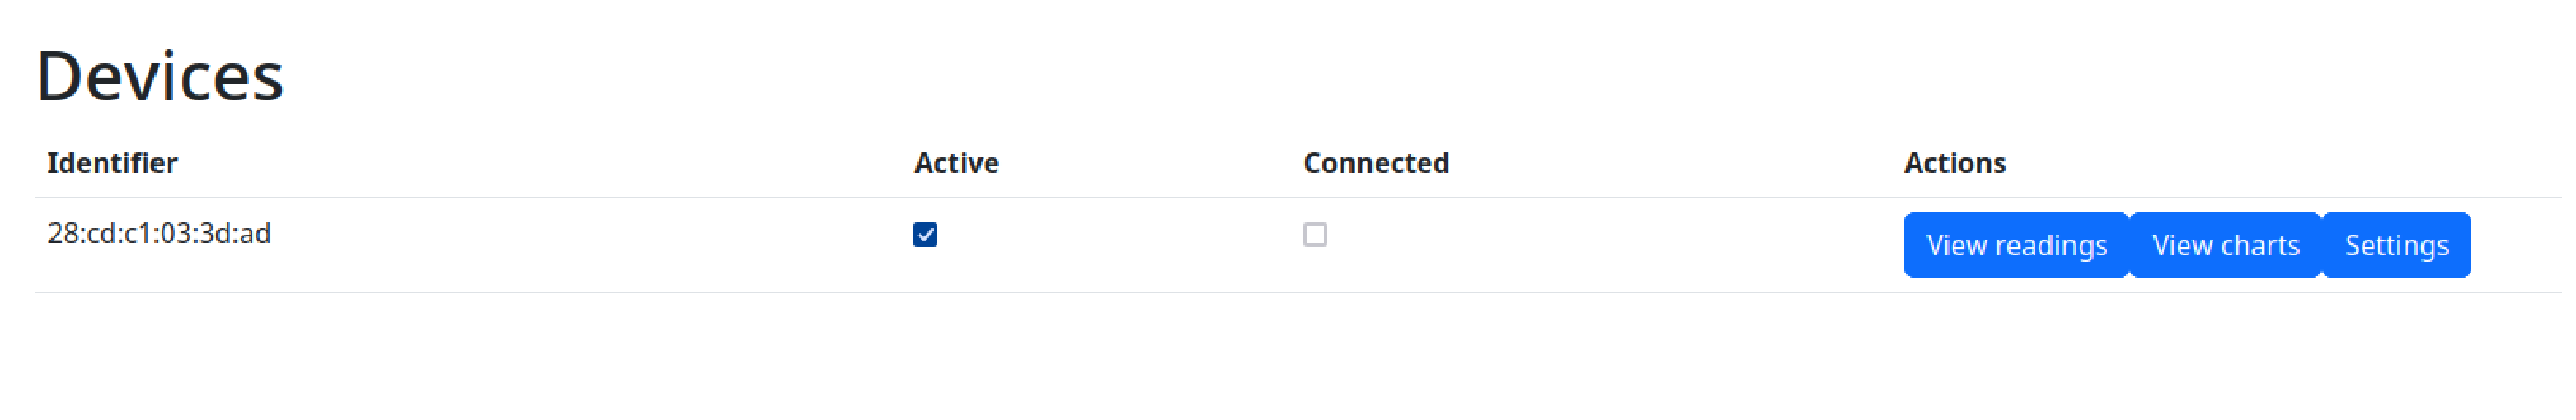
\includegraphics[width=\textwidth]{connect_dev}
  \caption{Nowe urządzenie na liście urządzeń}
  \label{test:connect_dev}
\end{figure}
Następnie aktywowano urządzenie, aby te mogło przesyłać odczyty. Natychmiastowo użytkownik
otrzymuje testową notyfikację oraz na widoku odczytów widoczne są utworzone odczyty.
Stan aplikacji zaprezentowano na Rys. \ref{test:readings}.
\begin{figure}[h!]
  \centering
  \includegraphics[width=\textwidth]{test_readings}
  \caption{Odczyty oraz notyfikacje po aktywacji urządzenia}
  \label{test:readings}
\end{figure}
